\section{Task II : Key Events}
\subsection*{Calculation Methods}
To identify key events, we will use the proportion of medals from these events among the whole medal tally as a main factor.

\[
P_{\text{total}} = \sum_{i=1}^{n} \frac{\text{M}_{ei}}{\text{M}_{tc}}
\]

This is the calculation formula related to PCA.

\[
\Sigma = \frac{1}{n-1} \mathbf{X}_{\text{c}}^T \mathbf{X}_{\text{c}} = \frac{1}{n-1} \sum_{i=1}^{n} \left( \mathbf{x}_i - \mu \right) \left( \mathbf{x}_i - \mu \right)^T
\]

where
\[
\Sigma \in \mathbb{R}^{d \times d} \text{ is the covariance matrix, } \mathbf{x}_i \text{ is the } i\text{th sample, and } \mu \text{ is the mean vector of the features.}
\]

\begin{figure}[htbp]
    \centering
    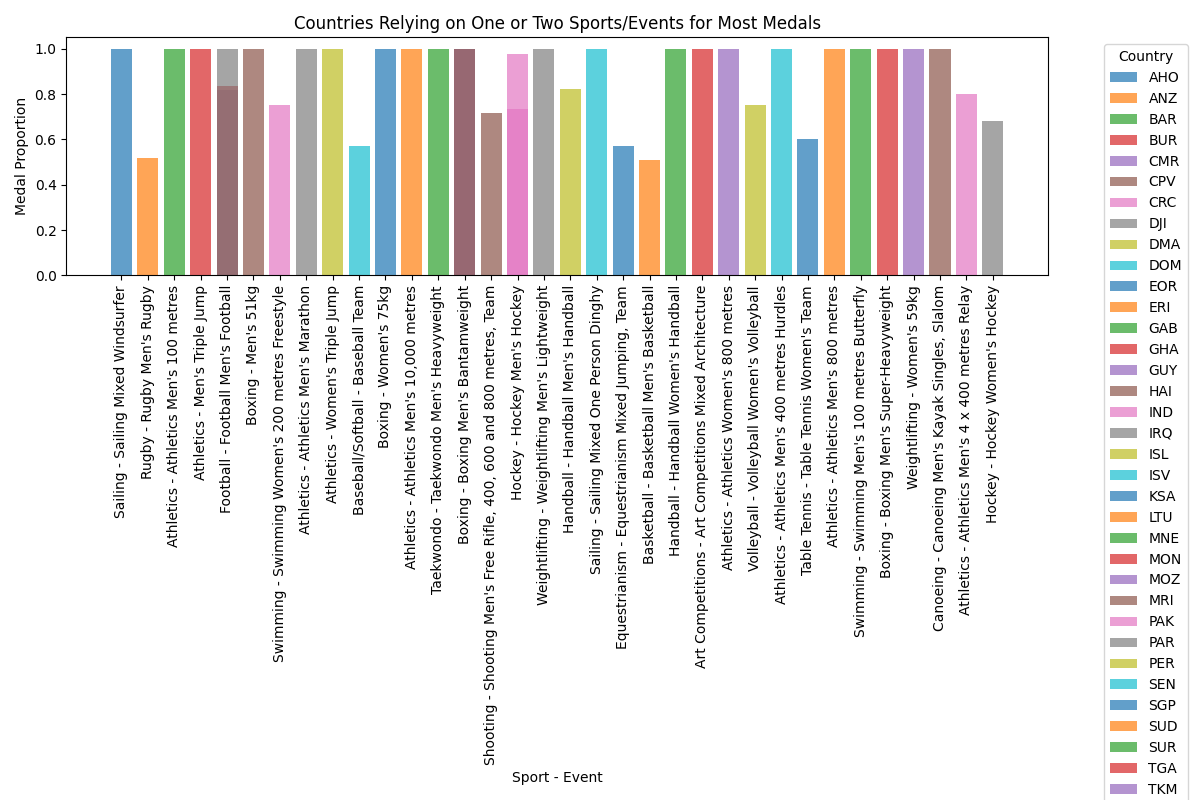
\includegraphics[width=1\textwidth]{./figures/Key_event.png}
    \caption{ Countries with biased medal distribution}
    \label{fig:Key_event}
\end{figure}

From this graph, we can see that many countries rely on one or two sports/events for their medal tally. This can be inspiring for the countries' Olympics committees.
If the home country doesn't choose some specific sports/events, such as long distance race for Kenya, it would be disastrous for those countries who are expert in these fields.
This push the committees to increase the variety of their countries participation fields.
